% Wei-Jin Huang -- Chinese academic CV (academic blue edition)
% Build: xelatex wei_jin_huang_cv_zh.tex
\documentclass[10pt,a4paper]{article}

\usepackage[a4paper,top=0.8cm,bottom=0.5cm,left=1.45cm,right=1.45cm]{geometry}
\usepackage{fontspec}
\usepackage{xeCJK}
\usepackage{microtype}
\usepackage{xcolor}
\usepackage{graphicx}
\usepackage{enumitem}
\usepackage{ragged2e}
\usepackage{fontawesome5}
\usepackage{tikz}
\usepackage[hidelinks]{hyperref}

% ---- fonts -----------------------------------------------------------------
\setmainfont{HelveticaNeueLTPro-Roman.otf}[
  Path = fonts/,
  BoldFont = HelveticaNeueLTPro-Md.otf,
  ItalicFont = HelveticaNeueLTPro-Roman.otf,
]
\setCJKmainfont{FandolHei-Regular.otf}[
  BoldFont = FandolHei-Bold.otf,
]

% ---- palette ---------------------------------------------------------------
\definecolor{ink}{HTML}{1F2937}
\definecolor{muted}{HTML}{667085}
\definecolor{primary}{HTML}{365A7C}
\definecolor{rule}{HTML}{D8DEE6}
\definecolor{soft}{HTML}{EEF3F7}
\color{ink}

\hypersetup{colorlinks=true,urlcolor=primary,linkcolor=primary}
\setlength{\parindent}{0pt}
\pagestyle{empty}
\linespread{1.07}

% ---- helpers ---------------------------------------------------------------
\newcommand{\cvsection}[1]{%
  \vspace{2pt}\par\noindent
  {\color{primary}\rule[-1pt]{3.2pt}{12pt}}\hspace{6pt}%
  {\bfseries\large\color{primary}#1}\par
  \vspace{2.5pt}{\color{rule}\hrule height 1pt}\vspace{3.5pt}}

\newcommand{\dt}[1]{{\bfseries\color{muted}\footnotesize #1}}
\newcommand{\me}[1]{{\bfseries\color{primary}#1}}
\newcommand{\venue}[1]{{\bfseries\color{primary}#1}}

\newcommand{\badge}[1]{%
  \tikz[baseline=(c.base)]{\node[fill=soft,text=primary,rounded corners=2.5pt,
    inner xsep=0pt,inner ysep=0pt,minimum width=1.45em,minimum height=1.45em,
    font=\bfseries\small](c){#1};}}

% publication block: number / title / authors / venue / summary / url
\newcommand{\pub}[6]{%
  \noindent
  \begin{minipage}[t]{1.55em}\vspace{1.5pt}\badge{#1}\end{minipage}\hspace{0.6em}%
  \begin{minipage}[t]{\dimexpr\linewidth-2.15em\relax}\vspace{0pt}
    \if\relax\detokenize{#6}\relax
      {\bfseries\color{ink} #2}\par
    \else
      \href{#6}{\bfseries\color{ink} #2}\par
    \fi
    {\small\color{muted}#3}\par
    \vspace{0.5pt}#4\par
    \if\relax\detokenize{#5}\relax\else
      \vspace{1pt}{\color{ink}{\bfseries\color{primary}简介：}#5}\par
    \fi
  \end{minipage}\par\vspace{1.5pt}}

\begin{document}
\justifying
\setlength{\parindent}{0pt}

% ============================ HEADER =======================================
\begin{minipage}[b]{0.79\textwidth}
  {\fontsize{25}{28}\selectfont\bfseries\color{ink} Wei-Jin Huang}\\[4pt]
  {\bfseries\color{primary} 博士研究生}{\color{muted}｜计算机科学与技术}\\[1.5pt]
  {\color{muted} 中山大学｜中国·广州}\\[5pt]
  {\footnotesize\color{primary}%
    \faEnvelope[regular]~\href{mailto:huangwj235@mail2.sysu.edu.cn}{huangwj235@mail2.sysu.edu.cn}\quad
    \faGlobe~\href{https://vkgo.github.io/}{vkgo.github.io}\\[2.5pt]
    \faGraduationCap~\href{https://scholar.google.com/citations?user=jMrU_JYAAAAJ}{Google Scholar}\quad
    \faGithub~\href{https://github.com/vkgo}{github.com/vkgo}\quad
    \faKaggle~\href{https://www.kaggle.com/carmencita}{carmencita}}
\end{minipage}\hfill
\begin{minipage}[b]{0.19\textwidth}
  \raggedleft
  {\setlength{\fboxsep}{0pt}\setlength{\fboxrule}{0.8pt}%
   \fcolorbox{rule}{white}{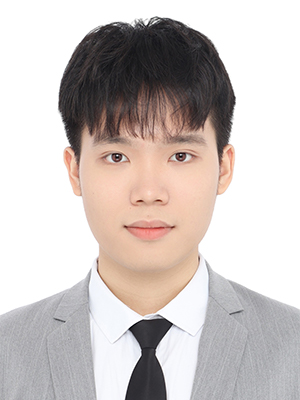
\includegraphics[height=2.85cm]{photo.jpg}}}
\end{minipage}

\vspace{6pt}
{\color{primary}\hrule height 1.5pt}
\vspace{2pt}

% ============================ SUMMARY ======================================
\cvsection{研究概述}
中山大学计算机科学与技术专业博士研究生，导师为郑伟诗教授。研究聚焦人形机器人学习与视频动作理解：
一方面从人类示范中学习具备物理可执行性的全身人—人形机器人交互策略，另一方面理解视频中的细粒度人体动作。
以（共同）第一作者身份在 CVPR、ICCV、ECCV 和 ACM MM 发表论文，致力于以严谨、可落地的研究推进具身智能。

% ============================ OPPORTUNITIES ================================
\cvsection{实习/合作意向}
让智能体在物理世界中感知、行动并持续学习，是迈向通用智能的重要挑战。围绕这一目标，我关注机器人策略的跨任务泛化，
尤其是如何使机器人在未见任务中理解目标、复用并组合已有技能。下一步值得探索的方向，是将 VLA、WAM、agentic planning
与持续学习机制相结合；在实习与合作中，我希望进一步利用第一视角人类数据和机器人持续交互经验，研究新任务上的组合泛化、
快速适应与失败恢复。

% ============================ EDUCATION ====================================
\cvsection{教育经历}
{\bfseries 博士｜计算机科学与技术} — 中山大学，中国·广州 \hfill \dt{2024.09 — 至今}\\
{\color{muted}\small 研究方向：人形机器人学习、视频动作理解}\\[2pt]
{\bfseries 工学学士｜网络工程} — 华南理工大学，中国·广州 \hfill \dt{2020.09 — 2024.07}\\
{\color{muted}\small 专业平均成绩排名：3/66}

% ============================ PUBLICATIONS =================================
\cvsection{代表性论文}
\pub
  {1}{ChoreoPlan: Hybrid Phrase Planning and Execution-Grounded Selection for Music-to-Humanoid Dance}
  {\me{Wei-Jin Huang}, Jianhong Fan, Hao Huang, Zhi-Wei Xia, Jun-Yi Deng, Yuan-Ming Li, Kun-Yu Lin, Wei-Shi Zheng}
  {\venue{ACM MM 2026}}
  {针对优质参考舞蹈经人形机器人控制后可能失稳的问题，ChoreoPlan 将节拍对齐的混合短语规划与基于离线控制器轨迹训练的
   Embodied Selector 相结合，优先选择兼具可执行性与语义一致性的候选动作。在 AIST++、FineDance 及 IsaacGym、MuJoCo
   上提升执行成功率、跟踪精度、节奏与语义保持能力，并迁移至 Unitree G1 实机。}
  {}

\pub
  {2}{Beyond Mimicry: Learning Whole-Body Human-Humanoid Interaction from Human-Human Demonstrations}
  {\me{Wei-Jin Huang}, Yue-Yi Zhang, Yi-Lin Wei, Zhi-Wei Xia, Juantao Tan, Yuan-Ming Li, Zhilin Zhao, Wei-Shi Zheng}
  {\venue{CVPR 2026}}
  {针对高质量人—人形机器人交互数据稀缺的问题，我们提出接触保持重定向流程 PAIR，利用大规模人人交互数据生成训练样本，
   并提出分层交互策略 D-STAR。在六项交互任务上取得先进水平的 75.4\% 平均成功率，且可迁移至真实 Unitree G1 人形机器人。}
  {https://cvpr.thecvf.com/virtual/2026/poster/37452}

\pub
  {3}{Modeling Multiple Normal Action Representations for Error Detection in Procedural Tasks}
  {\me{Wei-Jin Huang}, Yuan-Ming Li, Zhi-Wei Xia, Yu-Ming Tang, Kun-Yu Lin, Jian-Fang Hu, Wei-Shi Zheng}
  {\venue{CVPR 2025}}
  {针对程序化任务中的异常检测依赖时间顺序或单一正常原型的问题，提出 AMNAR，自适应预测所有可能的下一步正常动作并重建其表示，
   与当前动作进行比较。在 EgoPER、HoloAssist 和 CaptainCook4D 上达到先进水平，较此前最佳方法提升 7.4\% EDA 与 6.5\% AUC。}
  {https://openaccess.thecvf.com/content/CVPR2025/html/Huang_Modeling_Multiple_Normal_Action_Representations_for_Error_Detection_in_Procedural_CVPR_2025_paper.html}

\pub
  {4}{Less Static, More Private: Towards Transferable Privacy-Preserving Action Recognition by Generative Decoupled Learning}
  {Zhi-Wei Xia, Kun-Yu Lin, Yuan-Ming Li, \me{Wei-Jin Huang}, Xian-Tuo Tan, Wei-Shi Zheng}
  {\venue{ICCV 2025}}
  {针对隐私保护动作识别在视频域变化下泛化不足的问题，提出 GenPriv，通过解耦静态与动态视频特征，并从静态特征中去除隐私敏感信息，
   实现兼顾隐私保护的强跨域动作识别能力。}
  {https://openaccess.thecvf.com/content/ICCV2025/html/Xia_Less_Static_More_Private_Towards_Transferable_Privacy-Preserving_Action_Recognition_by_ICCV_2025_paper.html}

\pub
  {5}{EgoExo-Fitness: Towards Egocentric and Exocentric Full-Body Action Understanding}
  {Yuan-Ming Li, \me{Wei-Jin Huang（共同第一作者）}, An-Lan Wang, Ling-An Zeng, Jing-Ke Meng, Wei-Shi Zheng}
  {\venue{ECCV 2024}}
  {提出 EgoExo-Fitness：包含 40 名受试者、1,276 组跨视角健身序列与 32 小时视频，由六台同步的第一与第三视角相机采集。
   数据集提供两级时间边界、自然语言点评和 1--5 分动作质量评分，支持细粒度、可解释的动作分析。}
  {https://doi.org/10.1007/978-3-031-72661-3_21}

% ============================ HONORS =======================================
\cvsection{荣誉与奖励}
\dt{2024}\hspace{0.7em}中山大学校长奖学金（前 5\%）\\[2.5pt]
\dt{2022}\hspace{0.7em}Kaggle H\&M 个性化时尚推荐竞赛，银牌（85/2952）\\[1.5pt]
\hspace*{2.05em}国家奖学金（1/66）\quad{\color{rule}\textbullet}\quad 腾讯奖学金一等奖（1/66）\\[2.5pt]
\dt{2021}\hspace{0.7em}Kaggle G2Net 引力波检测竞赛，银牌（57/1219）

\end{document}
